The implemented Virtual Personal Assistant combines state-of-the-art technologies for speech recognition (Whisper), chatbot functionality (BanglaBERT), and Bangla text-to-speech capability.
The system effectively comprehends user speech input in the Bengali language and demonstrates the ability to accurately extract relevant answers from provided contexts using the BanglaBERT model.
This extracted information is then vocalized in Bengali through text-to-speech synthesis.

The system's performance showcases its proficiency in understanding spoken Bengali input and subsequently utilizing BanglaBERT to locate and articulate correct responses.
Although the system has not been extensively customized or fine-tuned to cater to specific user demands, the successful implementation serves as a proof-of-concept that customization is possible.
This adaptability suggests potential for tailoring the system to fulfill a wide array of user requirements.

As evidence of functionality, a provided screenshot [Figure \ref{fig:result}] displays a dialogue interaction, wherein the user speaks in Bengali and the system responds appropriately.
This interaction underscores the system's real-time capabilities in processing user input, deciphering context, and generating coherent spoken Bengali output.

In summary, the Virtual Personal Assistant effectively integrates prevalent technologies to comprehend and respond to Bengali speech inputs, demonstrating its potential for customization to meet diverse user needs.

\begin{figure}
    \centering
    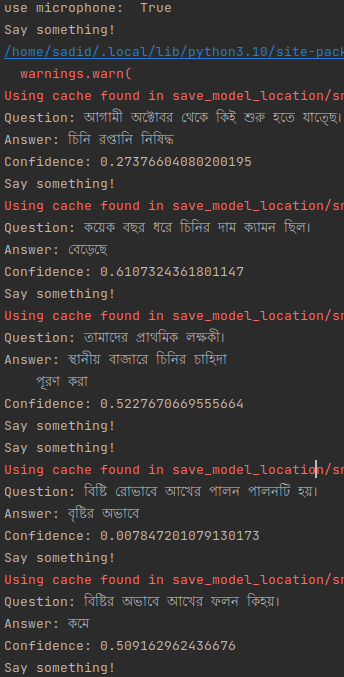
\includegraphics[width=0.47\textwidth]{result}
    \caption{Screenshot—Output of the program}\label{fig:result}
\end{figure}
